\section{Implementation}

Together with his paper, Sigg has written a small library implementing ray-casting of spheres and cylinders, 
which is available from his web site \cite{siggsite}.
The shader files included with this implementation have been written using the arbvp1/fp1 assembly-like instruction sets and are heavily optimized.
This makes them fairly difficult to decipher, limiting their use as reference for our own implementation.

Our implementation was done using Nvidia's high-level GPU programming language Cg.
Aside from the deviations we described in the previous section, we have largely followed the methods from Sigg's paper.
Occasionally, Sigg's implementation has been used as reference and support.

We have implemented nearly all the features mentioned in Sigg's paper.
This includes the bounding box computation and ray-casting of both spheres and cylinders (Figs. \ref{f:spheres}, \ref{f:cylinders}).
Using positions and normals obtained by ray-casting, a Phong shading term is evaluated for each fragment.
Deferred shading has been implemented, as well as rendering of silhouette and crease outlines (Fig. \ref{f:outlines}).

\begin{figure}[!ht]
\centering
\subfloat[Spheres only]{\label{f:spheres}\resizebox{50mm}{!}{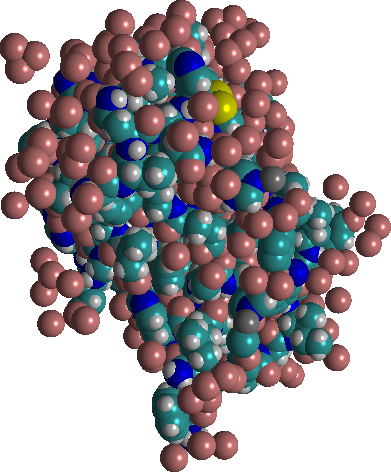
\includegraphics{img/spheres.png}}}
\subfloat[Spheres and cylinders]{\label{f:cylinders}\resizebox{50mm}{!}{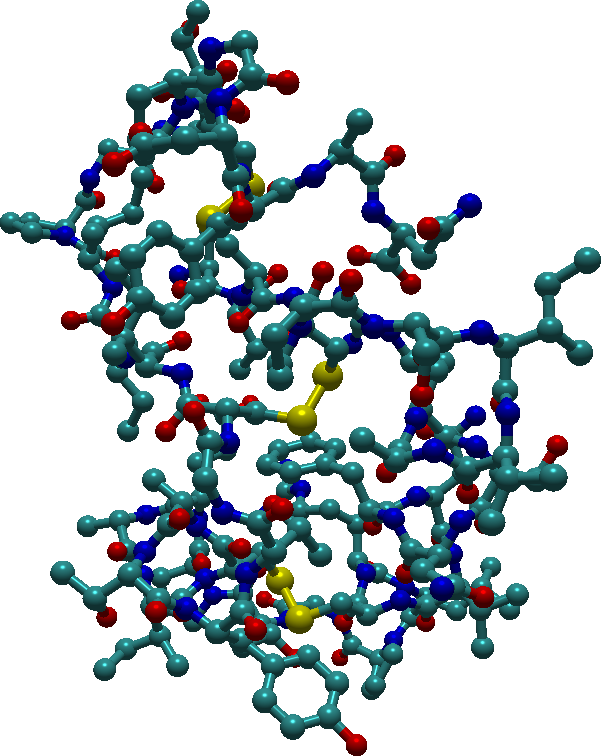
\includegraphics{img/cylinders.png}}}
\subfloat[Silhouette outlines]{\label{f:outlines}\resizebox{50mm}{!}{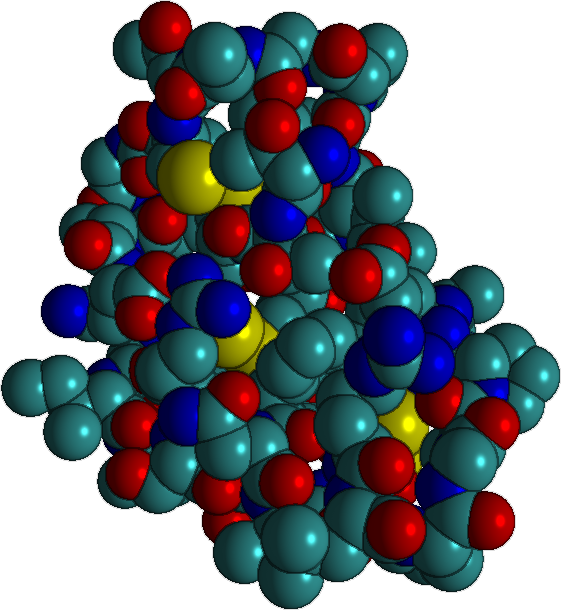
\includegraphics{img/outlines.png}}}
\caption{\em Ray-casted renderings of several data sets with varying effects}
\label{f:renderings}
\end{figure}

In his implementation, Sigg also applies soft shadow mapping to the models.
Implementing shadow mapping takes a considerable amount of time and is not the purpose of this exercise, 
so this step has been omitted in our implementation.

\subsection*{Deferred shading}

In addition to standard direct shading, a rendering path that uses deferred shading has also been implemented.
It works pretty much like any implementation of deferred shading, with one exception:
instead of storing a fragment's depth value in the geometry buffer, its value of the interpolation factor $\mu$ is stored instead.
This allows the eye-space surface position to be computed in the same way as it is for direct shading.

Silhouette lines are added as an option to improve the distinction of each quadric, using the geometry buffers stored for deferred shading.
It is implemented by applying a Sobel edge detection filter to both the normals and the depth values.
Although we only store the value of $\mu$ in the geometry buffers, it can be used as an approximation of the depth value and provides
a good enough gradient for generating silhouette lines.
Applying edge detection to the normals causes intersections between quadrics, or creases, to also be marked with an outline.
The strength of these two types of outlines can be tuned through several parameters in the deferred shading fragment shader.

\subsection*{Optimization}
Both the vertex shaders and the fragment shaders have been optimized to decrease the number of instructions per shader program, 
in order to increase their performance.

One interesting optimization for both shaders, inspired by Sigg's implementation, involves some modifications to the
quadratic formula, to essentially perform several multiplications and divisions in a single step. 

The most common notation of the quadratic formula is as follows:
\[
x = \frac{-b \pm \sqrt{b^2 - 4ac}}{2a}
\]
We can define the following helper variables:
\begin{eqnarray*}
b' & = & \frac{b}{2a}\\
c' & = & \frac{c}{a}\\
\end{eqnarray*}
These values can be computed on the GPU with a single instruction by dividing a temporary vector $(\frac{b}{2}, c)^T$ by $a$.

Then:
\begin{eqnarray*}
b'^2 - c' & = & \frac{b^2}{4a^2} - \frac{c}{a}\\
 & = & \frac{b^2}{4a^2} - \frac{4ac}{4a^2}\\
 & = & \frac{b^2 - 4ac}{4a^2}\\
\end{eqnarray*}
This is enough to determine if the discriminant is positive, negative or zero and so whether a fragment should be discarded or not.

The rest of the quadratic formula can be solved as follows:
\begin{eqnarray*}
\sqrt{b'^2 - c'} & = & \sqrt{\frac{b^2 - 4ac}{4a^2}}\\
 & = & \frac{\sqrt{b^2 - 4ac}}{2a}\\
\end{eqnarray*}
The entire quadratic formula can thus be written as:
\begin{eqnarray*}
x & = & -b' \pm \sqrt{b'^2 - c'}\\
 & = & -\frac{b}{2a} \pm \frac{\sqrt{b^2 - 4ac}}{2a}\\
\end{eqnarray*}
Simplifying the quadratic formula to this form saves a significant number of multiplications, thus reducing the number of instructions necessary
to compute its solutions.

\subsection*{Cylinders}

Cylinders differ from spheres insomuch that they do not look the same from all angles and they do not have a bounded volume.
These differences are also reflected in their respective shaders.

The ray-casting portion done in the fragment shader is mostly similar for cylinders. 
The only differences are that the surface normal does not equal the surface position in parameter space, 
but instead the normal equals the parameter-space position with its z-coordinate set to $0$.
Also, a cylinder needs to be capped, so an additional test is done that discards fragments outside the parameter-space unit cube.

The variance matrix generated in the vertex shader is very simple for spheres, because it involves only scaling and translation;
rotation is ignored because spheres appear the same from all angles. 
For cylinders on the other hand, rotation is an important factor, making the variance matrix and its inverse that much more complex to compute.

The bounding box computation for cylinders is also very different. 
Because a cylinder is an infinite volume, it needs to be capped by the unit cube in parameter space to be useful for rendering.
A cylinder's bounding box is computed by taking the union of the bounding boxes of the two end caps.

Currently, the vertex shader for cylinders is not optimized at all. 
At the time of writing, the vertex shader compiles to 166 instructions, compared to 35 instructions for spheres.
Also, the bounding box computation has not been thoroughly tested and might not be completely correct.

Because of the limitations of the cylinder implementation, its inclusion is considered to only be a proof of concept. 
Cylinders have not been taken into account in the benchmarks.
